\documentclass{beamer}


\mode<presentation>

\usetheme{Warsaw}     

\usecolortheme{default} 
\usefonttheme{default} 
\setbeamertemplate{navigation symbols}{}
\setbeamertemplate{caption}[numbered]
\usepackage{ragged2e}
\usepackage[english]{babel}
\usepackage[utf8]{inputenc}
\usepackage{hyperref}
\usepackage{amsmath,bm}
\usepackage{upgreek}
\usepackage{multicol}
\usepackage{textcomp}
\usepackage{bbm}
\usepackage[normalem]{ulem}
\usepackage{graphicx}
\usepackage{amssymb}
\usepackage{mathtools}
\usefonttheme{professionalfonts}
 

\title[Multi Layer Perceptron]{Multi Layer Perceptron}
\author{M. Saiful Bari}


\begin{document}

\begin{frame}	
  \titlepage
\end{frame}




\begin{frame}

    \frametitle{Table of Contents}
	\begin{multicols}{2}
	    \tableofcontents
	\end{multicols}

\end{frame}



\section{Introduction}
\subsection{Defination}
\begin{frame}
    \frametitle{Introduction}
	\begin{block}{}
		\small \textcolor{red}{Feedforward Neural Network} \textcolor{blue}{aka} \textcolor{red}{(\textbf{M})ulti-(\textbf{L})ayer (\textbf{P})erceptron (\textbf{MLP})}
	\end{block}
	Series of \textbf{\textcolor{blue}{logistic regression}} models \textbf{\textcolor{red}{stacked}} on top of each other, with the \textbf{final layer} being either another \textbf{\textcolor{blue}{logistic}} or a \textbf{\textcolor{blue}{linear regression}} model.

\end{frame}



\subsection{Example}
\begin{frame}
    \frametitle{MLP : Example}
	Assume, we have \textbf{two layers}, and we are solving a \textbf{\textcolor{blue}{regression problem}}, the model has the form,
	\begin{align*}
	    p(y|\bm{\mathsf{x},\theta}) &= \mathcal{N}(y|\bm{\mathsf{w^{T}z(x)}},\sigma^{2})\\
	    \bm{\mathsf{z(x)}} &= g(\bm{\mathsf{Vx}}) = [g(\mathsf{v_{1}^{T}x)}, ... ,g(\mathsf{v_{H}^{T}x)}]
	\end{align*}
	where, 
	\begin{itemize}

		\item $g$ is a non-linear \textcolor{blue}{activation} or \textcolor{blue}{transfer function} (commonly the \textcolor{blue}{logistic function}).\\
		\item $\bm{\mathsf{z(x) = \phi(x, V)}}$ is called the hidden layer (a deterministic function of the input)
		\item $H$ is the number of \textcolor{red}{hidden units}.
		\item $V$ is the \textbf{weight matrix} from the inputs to the hidden nodes
		\item $\mathsf{w}$ is the \textbf{weight vector} from the hidden nodes to the output
	\end{itemize}

\end{frame}


	
\begin{frame}
    \frametitle{MLP}
	\begin{align*}
	    p(y|\bm{\mathsf{x},\theta}) &= \mathcal{N}(y|\bm{\mathsf{w^{T}z(x)}},\sigma^{2})\\
	    \bm{\mathsf{z(x)}} &= g(\bm{\mathsf{Vx}}) = [g(\mathsf{v_{1}^{T}x)}, ... ,g(\mathsf{v_{H}^{T}x)}]
	\end{align*}
	\begin{block}{}
		\centering
		\textcolor{red}{It is important that $g$ be nonlinear, otherwise the whole model collapses into a large linear regression model of the form
$\bm{\mathsf{y = w^{T}(Vx)}}$}
	\end{block}
	\begin{block}{}
		One can show that an \textbf{MLP} is a \textbf{\textcolor{red}{universal approximator}}, meaning it can model any suitably \textbf{\textcolor{red}{smooth function}}, given enough \textbf{hidden units}, to any \textbf{\textcolor{red}{desired}} level of accuracy. \textbf{(Hornik 1991)}
	\end{block}
\end{frame}




\begin{frame}
	\frametitle{MLP : Example}
	To handle binary classification, we pass the output through a sigmoid, as in a GLM.
	$$p(y|\bm{\mathsf{x,\theta}}) = \mathrm{Ber}(y|\mathrm{sigm}(\bm{\mathsf{w^{T}z(x)}}))$$
	We can easily extend the MLP to predict multiple outputs. For example, in the regression case, we have
	$$p(y|\bm{\mathsf{x,\theta}}) = \mathcal{N}(\bm{\mathsf{y}|W\phi} (\bm{\mathsf{x,V}}),\sigma^{2}\bm{I})$$
	
\end{frame}



\begin{frame}
    \frametitle{MLP : Example}
	\begin{figure}
    	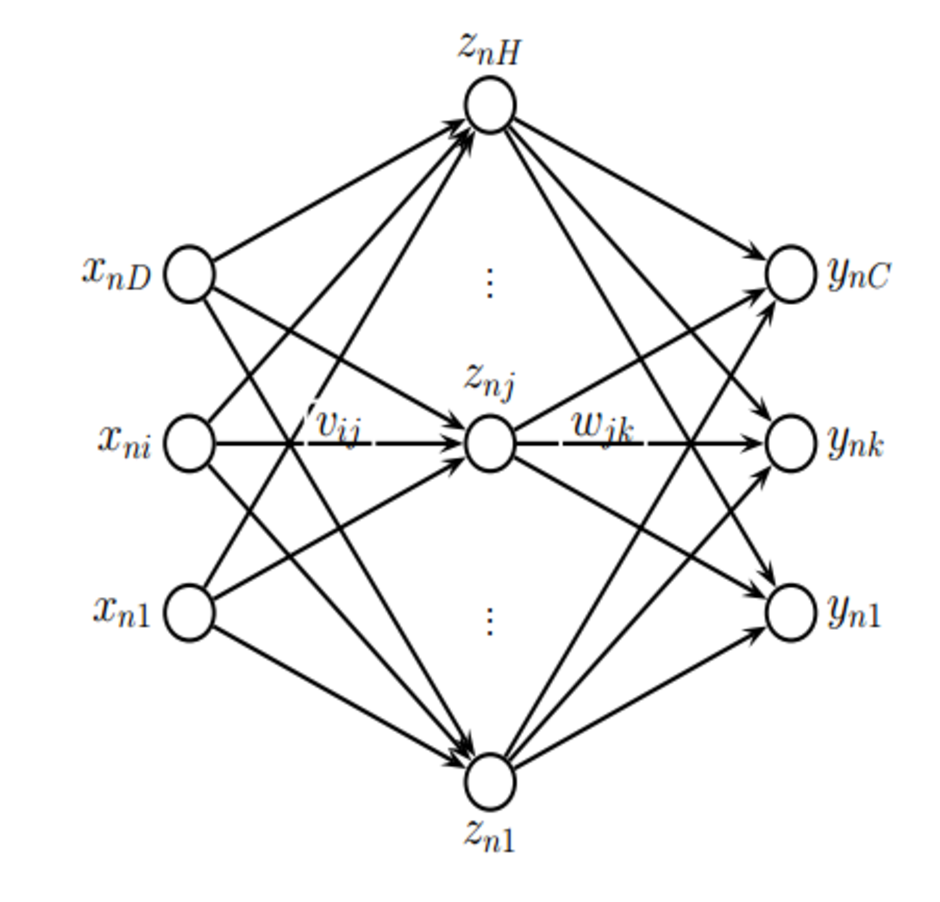
\includegraphics[scale=.4]{./Images/nn.pdf}
    	\caption{A neural network with one hidden layer}
	\end{figure}
\end{frame}


\begin{frame}
    \frametitle{MLP : Example}
	
	If we add \textbf{\textcolor{red}{mutual inhibition arcs}} between the \textbf{output units}, ensuring that only one of them turns on, we can enforce a \textbf{\textcolor{red}{sum-to-one}} constraint, which can be used for \textbf{multi-class classification}. 
	$$ p(y|\bm{\mathsf{x, \theta}}) = \mathrm{Cat}(y|\mathcal{S}(\bm{W\mathsf{z}(\mathsf{x})})$$

\end{frame}



\section{The Backpropagation Algorithm}
\begin{frame}
    \frametitle{The Backpropagation Algorithm}
	
    \begin{itemize}
    	\item Unlike a Generalized Linear Model\textbf{(GLM)}, the Negative Log Likelihood\textbf{(NLL)} of an MultiLayer Perceptron\textbf{(MLP)} is a \textbf{\textcolor{blue}{non-convex}} function of its parameters.
    	\item We can find a \textbf{\textcolor{red}{locally optimal}} ML or MAP estimate using \textbf{\textcolor{red}{standard gradient-based optimization}}
methods.
		\item \textbf{MLP}s have lots of parameters, they are often trained on very large data sets.
		\item \textbf{GLM}s are usually fit with IRLS, which is a second-order offline method
		
    \end{itemize}


\end{frame}



\end{document}